\documentclass[a4paper]{article}

\usepackage{amsthm}
\usepackage{amsmath}
\usepackage{amsfonts}
\usepackage{caption}
\usepackage{subcaption}
\usepackage{graphicx}
\usepackage{float}
\usepackage[english]{babel}
\usepackage[colorinlistoftodos]{todonotes}
\usepackage[colorlinks=true, allcolors=blue]{hyperref}

\newtheorem{definition}{Definition}
\newtheorem{theorem}{Theorem}

\title{Networks and Communities}
\author{Joshua Mankelow --- 1902186}

\begin{document}
\maketitle

\begin{abstract}
    Networks are an example of a rigorous model for analysing and understanding real world complex systems. A very important quality of these network models is the naturally emergent community structure. Community detection allows us to identify clusters in the network that are well connected amongst eachother. If a network is being used to model a real world system then finding this structure has many implications about the behaviour of the system. For example, predicting the structure of a network after a change in dynamics. In this essay I will discuss some simple methods for community detection and the applications of community structure to the analysis and understanding of real world complex systems. \\
\end{abstract}

\newpage

\tableofcontents

\newpage

\section{Introduction to Networks}\label{sec:Introduction to Networks}
\todo[backgroundcolor=magenta]{Introduce Network Theory}
Networks in the technical sense are analogous to networks in the nontechnical sense - a collection of objects paired with a number of connections that can link any two objects. \emph{Networks: An Introduction} by \emph{Mark Newman} lists \emph{Technological Networks}, \emph{Social Networks}, \emph{Information Networks} and \emph{Biological Networks} as different systems that are modelled by the technical interpretation of a network.\cite[Contents]{newman10}. A brief example of a network would be something like the following: Imagine you and your friends are represented as dots (nodes or vertices) on a piece of paper. Then if any two people are friends, the dots representing those people are connected by a line (edge). If you then repeat this process by asking your friends to list all their friends and so on, you will end up with a simple model of a \emph{social network}.

As one might imagine, now that we have this model it's easy to be curious about any structure that emerges that we can detect and abuse to develop an understanding of the real world system that we are representing. The structure that this essay will explore is that of \emph{communities}. Vaguely speaking, communities are subsets of a network that are \emph{densely connected} amongst themselves. I.e. there is some notion of any node within a community being more closely connected to other nodes in the community than nodes outside the community in the average case. Before we dive into the details of communities and detecting them, I wish to provide some motivation by way of example of the kinds of situations that networks can arise and why they are the natural model for the related systems.

\subsection{Social Networks}\label{sec:Social Networks}
\todo[backgroundcolor=orange]{Models of Networks}
To better illustrate the simple notion of a social network mentioned above, I will introduce the canonical network theory example of \emph{Zachary's Karate Club}. Zachary's Karate Club is a dataset where "The data was collected from the members of a university karate club by Wayne Zachary in 1977.  Each node represents a member of the club, and each edge represents a tie between two members of the club."\cite{konect:2017:ucidata-zachary}. BLAH BLAH Zachary woow look it becomes bipartite if you remove only a few nodes etc.

\begin{figure}
    \begin{center}
        \begin{subfigure}[b]{0.45\textwidth}
            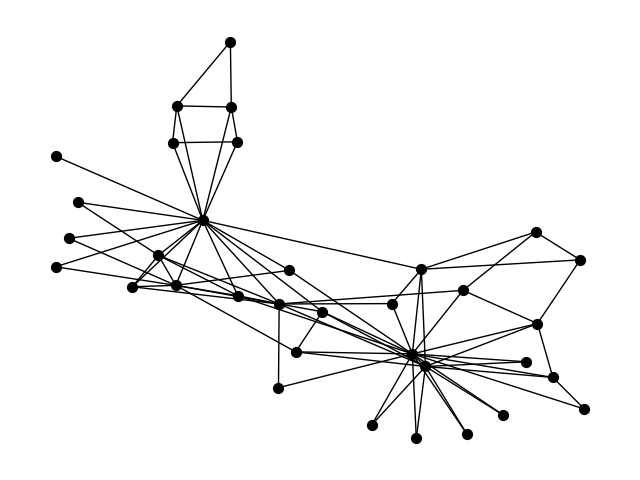
\includegraphics[width=\textwidth]{img/zachary_spring}
            \caption{Spring Layout}
            \label{fig:zachary_spring}
        \end{subfigure}
        \begin{subfigure}[b]{0.45\textwidth}
            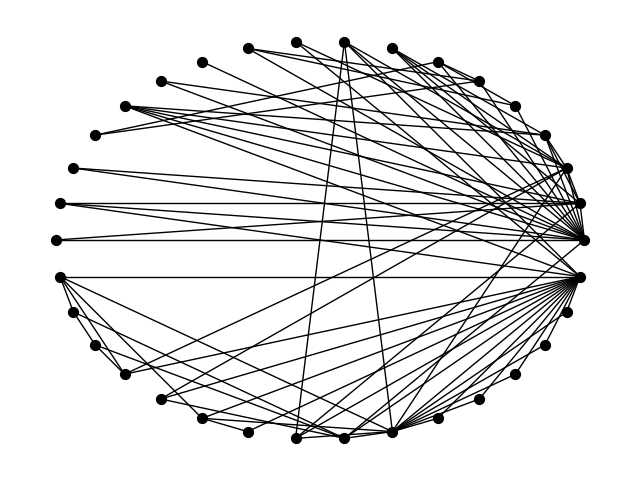
\includegraphics[width=\textwidth]{img/zachary_circle}
            \caption{Circle Layout}
            \label{fig:zachary_circle}
        \end{subfigure}
    \end{center}
    \caption{Two renderings of the Zachary Karate Club network using data from KONECT.cc\cite{konect:2017:ucidata-zachary} and a Python library NetworkX\cite{SciPyProceedings_11}}
    \label{fig:yeet}
\end{figure}

\subsection{Technological Networks}\label{sec:Technological Networks}
\subsection{Information Networks}\label{sec:Information Networks}
\subsection{Biological Networks}\label{sec:Biological Networks}

\todo[backgroundcolor=red]{Definition of a Network}
\todo[backgroundcolor=red]{Different Types of Network}

\newpage

\section{Properties of Networks}\label{sec:Properties of Networks}
\todo[backgroundcolor=red]{Interesting Properties of Networks}

\newpage

\section{Community Detection}\label{sec:Community Detection}
\todo[backgroundcolor=red]{SEC: Introduction to Community Detection}
As allured to in the previous chapters, detecting communities is of great interest and as such there a number of ways to do it. The process of community detection involves analysing the network and finding groups of nodes in the network that are more densely connected amongst themselves than they are to the rest of the network. This notion forms the basis for most community detection methods and algorithms. However, it turns out that it's difficult to come up with a good definition of a community. According to Fortunato, ``In most cases, communitys are algorithmically defined, i.e. they are just the final product of the algorithm without a precise \emph{a priori} definition."\cite[84]{fortunato} In this section, we will discuss the notions of ``community" that underpin a number of interesting methods in community detection before going into detail about the algorithms themselves.

\todo[backgroundcolor=red]{SEC: Background for Community Detection}

% \todo[backgroundcolor=red]{SEC: Traditional Methods of Community Detection}
%
% \todo[backgroundcolor=red]{SEC: Spectral Methods of Community Detection}

\todo[backgroundcolor=red]{SEC: Methods of Community Detection}

\subsection{Louvian Community Detection}

\subsection{Surprise Community Detection}

\subsection{Leiden Community Detection}

\subsection{Walktrap Community Detection}

\newpage

\section{Applications of Community Detection}\label{sec:Appliations of Community Detection}
In this section, we explore some applications of community detection. We will start with the simple example of Zachary's Karate Club and build up to more complicated examples.

\subsection{Zachary's Karate Club}
To add more to the context already introduced in Section \ref{sec:Social Networks}, the karate club that Zachary studied had two main leaders who are referred to in the paper as ``Mr Hi" and ``John A". Due to some inter-personal politics, members of the club ended up becoming part of a faction that was politically aligned with one of the primary leaders. After a period of in-fighting, the club split into two distinct groups. Zachary collected all the data relating to this including information on how often any two members of the group interacted, which leader they were factionally affiliated with and which group each member was a part of post-fission. Using this data, Zachary built a model that knew how much any two particular members interacted, but had no knowledge of their factional affiliations. After developing this model, Zachary was interested in the following two hypotheses:

\begin{enumerate}
    \item Can we predict the political affiliation of any member of the club pre-fission?
    \item Can we predict which club any member will join after the split?
\end{enumerate}

Zachary chose to model this problem as a network flow problem so that he could use the \emph{max-flow min-cut theorem} and the \emph{Ford-Fulkerson algorithm}\cite{ford_fulkerson_1956} to test his hypotheses. The max-flow min-cut theorem states that the maximum flow across a network is equal to the capacity of the minimum cut and the Ford-Fulkerson algorithm is a deterministic method for finding the minimum cut. Using this model we can rephrase the above two hypotheses:

\begin{enumerate}
    \item The minimum cut of the network should separate those factionally affiliated with Mr Hi from those factionally affiliated with John A.
    \item The minimum cut of the network should separate those who choose to join Mr Hi's club after the split from those who choose to join John A's club after the split.
\end{enumerate}

After running the Ford-Fulkerson algorithm on the data, Zachary achieved results that correctly predicted 34 out of 34 faction memberships and 33 out of 34 club memberships. The notable exception being individual number 9 who reportedly joined Mr Hi's club so as not to miss out on a black belt which they would have had to give up on if they'd joined John A's group. Figure \ref{fig:zachary_results} shows Zachary's full results.

\begin{figure}
    \begin{center}
        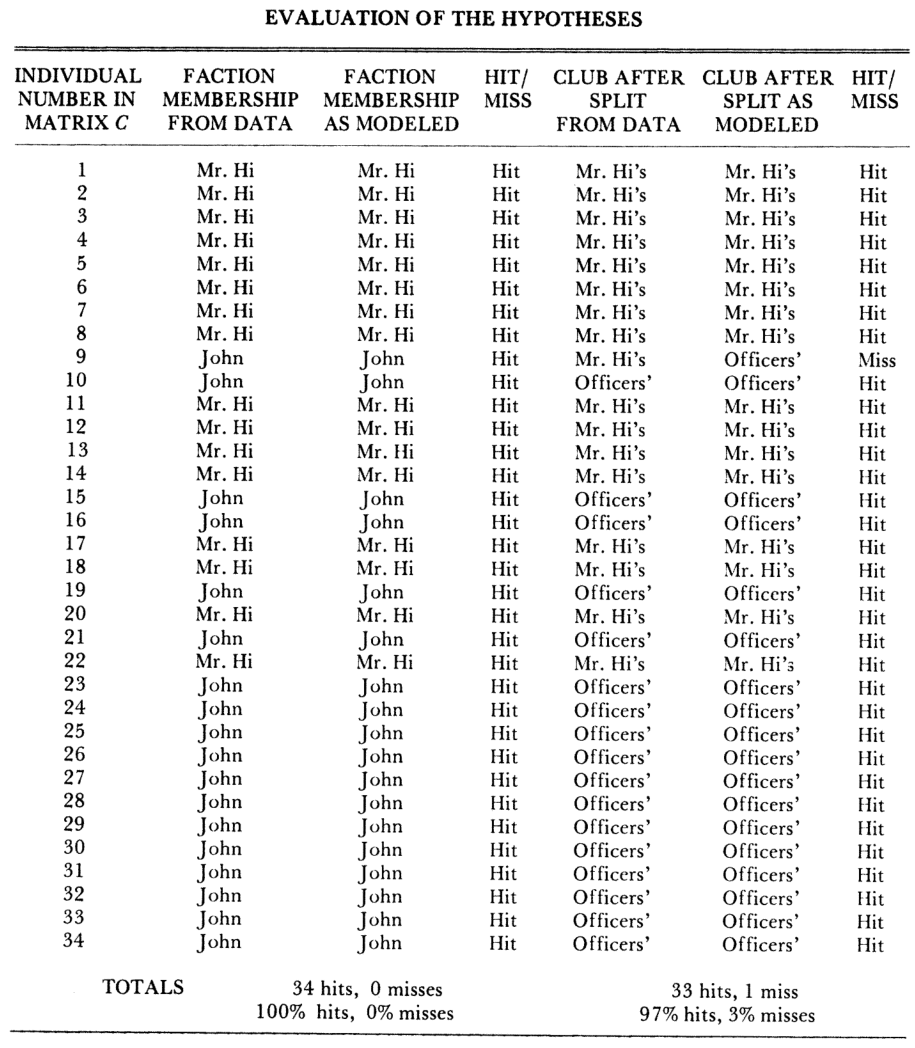
\includegraphics[width=0.95\textwidth]{img/zachary_results}
    \end{center}
    \caption{The full results from Zachary's investigation into using the Ford-Fulkerson minimum-cut algorithm to predict social and political alignments.\cite{konect:ucidata-zachary}}
    \label{fig:zachary_results}
\end{figure}

This is a prime example of the predictive power of community detection --- knowing nothing about the inter-group politics, Zachary was able to \emph{very} accurately predict the way the club interacted and split after a dispute.

\subsection{Epidemic Spreading and Community Structure}
From experience, we understand that community structure might make a difference to the spreading of a virus or disease through a population.\footnote{This wouldn't be an essay written in the 2020s without mentioning epidemic processes}. Until recently, the idea of analysing the difference in epidemic propagation between networks with and without communities remained nearly untouched. A paper by Huang and Li published in 2007\cite{Huang_2007} investigated the difference between epidemic spreading in scale-free networks with and without community structure. Recall from Section \ref{sec:Degree Distribution} that scale free networks have a degree distribution that rougly follows a power law. Further recall that scale-free networks are interesting because they represent a plethora of real world complex systems.

Huang and Li's method involves creating a number of realisations of scale-free networks (SFNs) and scale-free networks with communities (SFcNs) and performing Monte Carlo simulations for each realisation using a Susceptible-Infected (or SI) model. This model works by labelling each member of the network either susceptible, where the member can be infected by the disease, or infected, where the member currently has the disease and can infect others. The probability with which any infected member does this is parameterised by the authors using $\lambda$.

To generate the networks, Huang and Li refer to a paper by previous paper by Li et. al.\cite{Li_2005} that provides a method for generating scale-free networks with a community structure. The method is as follows:

\begin{enumerate}
    \item Initialisation: Choose $M \geq 2$ as the number of communities and $m_0 > 1$ the number of fully connected nodes in each community. Then add a link between every pair of communities so that there are a total of $M(M-1)/2$ inter-community links. These links are uniformly randomly assigned to nodes inside each community. \\
    \item Growth: In each iteration, we add a new node to a uniformly randomly selected community. This new node will be uniformly randomly connected to $1 \leq m \leq m_0$ nodes in the same community and with a probability $\alpha$ it will be connected to $1 \leq n \leq M$ nodes in the other $M - 1$ communities. \\
    \item Preferential attachments
    \begin{enumerate}
        \item Intra-community attachments: The probability of a new node being connected to a node $i$ in community $j$ is depends on the inner-degree $s_{ij}$ which is the number of intra-community links connected to $i$. The dependence is as follows
            $$ \Pi(s_{ij}) = \frac{s_{ij}}{\sum_ks_{kj}}. $$
        \item Inter-community attachments: Similarly to before, the probability of a new node being connected to a node $i$ in community $k$ depends on the inter-degree $l_{ik}$ which is the number of inter-community links connected to node $i$. This dependence is as follows
            $$ \Pi(l_{ik}) = \frac{l_{ik}}{\sum_{\substack{m, n \\ n \not = j}} l_{mn}} $$
    \end{enumerate}
\end{enumerate}

When the above is repeated for enough iterations, we get at SFcN with $N$ nodes and $M$ communities. To understand how strong the community structure generated by this method is, Huang and Li use the definition of modularity proposed by Newman and Girvan (see Section \ref{sec:qfs and modularity}). Using this measure of modularity and some results from \cite{Li_2005} we can obtain the modularity in terms of the parameters for the algorithm:

$$ Q = \frac{m}{m + \alpha n} - \frac{1}{M}\left(\frac{m + 2\alpha n}{m + \alpha n}\right)^2 $$

Thus, the authors fix the values of $m$ and $n$ and adjust the values of $\alpha$ to get networks with various strengths of community structure. Of course, for a fair test, the authors need a SFN with precisely the same degree distribution as the SFcN. Thus they perform a series of \emph{Monte Carlo vertex switching} steps on the SFcN to generate such a SFN. A single switching step involves taking a pair of links $\{A, B\}$ and $\{C, D\}$ and switching the ends to get $\{A, D\}$ and $\{C, B\}$. This switch is only performed if it doesn't form any multiple or self links. To ensure that there's enough mixing, the authors switch a total of $5M$ pairs of links. Clearly this process preserves the degree distribution. After all this set up, the authors then run the aforementioned Monte Carlo simulations for 30 different values of $\alpha$ and for each value of $\alpha$ they simulated 500 different initial conditions with one node chosen at random to be infected. The results from these simulations show that community structure has an impact on the spreading of the disease. Figure \ref{fig:si} shows the results for $\alpha = 0.01$ which gives a modularity $Q \approx 0.845$. In order from top left to bottom right, the plots represent the following things:

\begin{itemize}
    \item the proportion of individuals that are infected at time $t$,
    \item the variability of the proporotion of individuals that are infected at time $t$,
    \item the average degree of infected nodes at time $t$,
    \item the variability of the average degree of infected nodes at time $t$.
\end{itemize}


\begin{figure}
    \begin{center}
        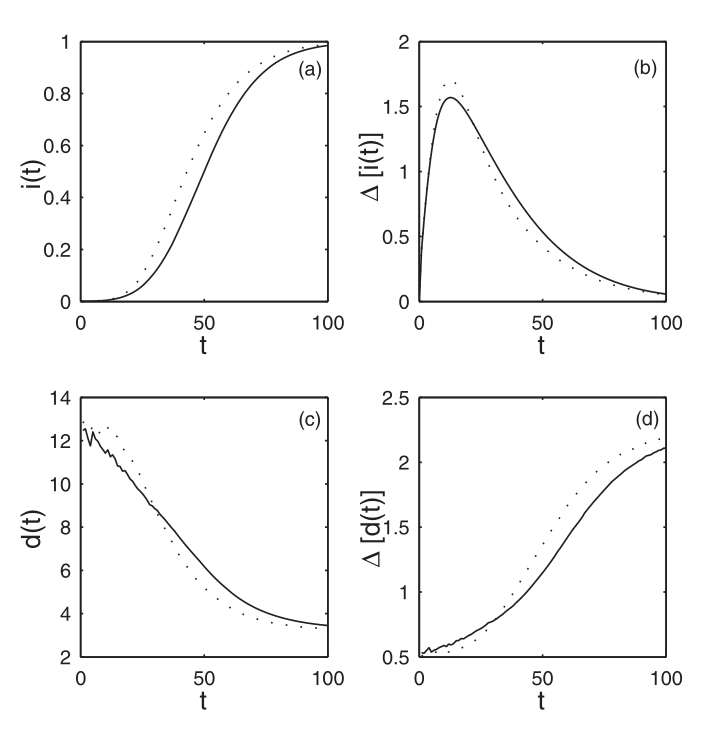
\includegraphics[width=0.95\textwidth]{img/si}
    \end{center}
    \caption{Results from Huang and Li's analysis of the difference in epidemic processes on SFNs and SFcNs for $\alpha = 0.01$, $\lambda = 0.03$ and $N = 2000$. SFNs are represented by the dotted line and SFcNs are represented by the solid line.}
    \label{fig:si}
\end{figure}

Observing the graphs we can see that SFNs behave differently to SFcNs. Most interestingly we can see that the proportion of infected individuals is \emph{lower} for SFcNs than it is for SFNs at any time $t$ and that the variability of the proportion of infected individuals peaks lower. This is significant because it informs our intuition that separating parts of the network results in slower transmission and lower infection proportions. Results like this are important because they have implications about how we adapt and inform our legislation when we're faced with real world problems.

\newpage

\section{Conclusion}
\subsection{Overview}
As a result of the topic being very computational in nature, community detection has scaled with computational power and this means that it is quite a young field. Despite this, a huge amount of research has been done on the topic thus far and Fortunato has done amazing work collating a large amount of the available information \cite{fortunato}. However, as always, there still remain open problems in the field. Recall Section \ref{sec:Community Detection}: In this section, we discussed that currently there is no strict definition of a community and that we typically define communities by the results of community detection algorithms and methods rather than having a definiton a priori. This appears to be the primary open problem in the field right now. Coming up with a strong and well supported definition of a community would let us better understand the quality of our methods and strategies for finding them. Failing this, the next best thing would be to design a comprehensive set of networks and suite of tests that we can give to community detection algorithms to test their efficacy. These networks and tests should obviously cover as many edge cases as possible to ensure that our algorithms work even for the most difficult to detect communities. 

It should further be noted that community detection and the ideas of community work both ways. Recall Section \ref{sec:Appliations of Community Detection}. In this section we discussed two applications of community detection: The Zachary Karate Club and Epidemic Spreading and Community Structure. In the first example, we are taking a given network and trying to analyse the underlying community structure, but in the second example we start with a network and show that by creating a community structure we gain some favourable characteristics. These two qualities of community detection when paired together make a very powerful framework and paradigm for investigating real world problems.


\subsection{Personal Learnings}
Throughout the course of writing this essay, I have developed a strong understanding of the foundations of research into community detection. What was most interesting to me was that there is no single strict definition of a community and instead we choose to define communities by the results of algorithms (Section \ref{sec:Community Detection}). This was a shock to me, but also unsurprising. A shock because I had expected that, given the utility and power of community detection in understanding real world phenomena, we would have a solid way to define what it is we're talking about. Unsurprising because networks are intuitively extremely complex on a large scale and, as such, identifying macroscopic properties such as community structure is understandably very hard. The most important personal learning from the writing of this essay was about quality functions and modularity. Of course it is required that there is some quantitative measure of the performance of an algorithm, but until researching them I had underappreciated the intricacy required to make such a measure. Take, for example, the Newman-Girvan modularity from Section \ref{sec:qfs and modularity}. This measure is not as simple as ``calculate the fraction of edges that go between communities". Instead there is a very deliberate design process and set of criteria that a quality function should meet such as normality (the property of being normalised) as well as the ability to omit trivial identifications of a community (such as putting all the nodes in the same community - this is technically a perfect detection of a community, but it doesn't help us understand the structure of the network in any way).

It should now be clear that networks and community detection are of great interest to the scientific community for their applications in modelling real world complex systems such as epidemic processes (Section \ref{sec:epidemics}) and social dynamics (Section \ref{sec:zachary_section}). Most importantly of all, we appreciate that community detection may be useful whenever you have a system that can be modelled as a network. For example: understanding the topology of the world wide web \cite{BARABASI200069} or how metabolic networks are organised \cite{Jeong2000}. All of this paired with the fact that our ability to solve large computational problems is ever increasing make communities a topic of interest for the future. I hope that the reader finds themselves with enough information to consider community structure when working on their next problem.

\newpage

\bibliographystyle{abbrv}
\bibliography{bib}

\end{document}
